\documentclass{article}

% Language setting
% Replace `english' with e.g. `spanish' to change the document language
\usepackage[english]{babel}
\usepackage{indentfirst}
% Set page size and margins
% Replace `letterpaper' with `a4paper' for UK/EU standard size
\usepackage[letterpaper,top=2cm,bottom=2cm,left=2cm,right=2cm,marginparwidth=1.75cm]{geometry}

% Useful packages
\usepackage{amsmath}
\usepackage{graphicx}
\usepackage[colorlinks=true, allcolors=blue]{hyperref}
\usepackage{float}%稳定图片位置
\usepackage{graphicx,subfig}%画图

\title{Entrepreneurship in Blockchain for Healthcare: \\A Solution for Plastic Surgery}
\author{Chongdan Pan}

\begin{document}
\maketitle

\begin{abstract}
Plastic surgery is a hot market that develops quite quickly with a large number of surgical procedures performed every year all over the world. However, at present, it's not a well-regulated industry because there are many cases where patients are injured or die from malpractice caused by unqualified surgeons or medicine, which may be unknown to the consumers. The intransparency has greatly increased the risk of taking plastic surgery. In this paper, we proposed a social business built up on a blockchain system. The system stores surgery data as traceable and immutable records. These data can provide a valuable and authenticated reference for other customers or help them manage personal data. What's more, the system can serve as a crowd-sourcing information platform in any industry where peer review is highly required.
\end{abstract}
\section{Introduction}
Healthcare is a part of a social business where blockchain can play a revolutionary role and benefit the public\cite{Business}. The industry has enormous stakeholders including patients, doctors, hospitals, and manufacturers who interact with each other in a complex way. In these intricate flows, trust is extremely critical because misbehaving or false information may put people's lives at risk. For a social business like healthcare, it's important to maintain trustworthy relationships and secure personal data management for stakeholders.
\par Luckily, blockchain was designed specifically for solving these pain points. Blockchain was introduced to the world as the fundamental technology of Bitcoin by Satoshi Nakamoto in 2008, aiming at keeping each transaction in a decentralized and immutable way\cite{Bitcoin}. In the past few years, Bitcoin has resisted multiple network attacks and reached a total market value of over 500 billion USD, proving the reliability and robustness of blockchain technology. For now, blockchain has evolved to be able to run smart contract "scripts that reside on the blockchain that allows for the automation of multi-step processes" \cite{SmartContract}. Compared to currency transactions, a smart contract can be a series of complex operations and save more states. For example, a smart contract can ensure that a doctor can only get the payment after the surgery is successfully completed. Since the stakeholders can only interact as the clear smart contract that everybody agrees on, we can trust that they're behaving well. 
\par Blockchain can be used to manage private data securely as well. The loss from a healthcare data breach is increasing rapidly in the past few years and people may be concerned that their private information is vulnerable to cyber attack\cite{breach}. Thanks to decentralization and cryptography, this won't be an issue for blockchain. To interact with a blockchain, the user only needs to generate a random private key and public key pair for verification. Then, unless knowing the private key, nobody can use a smart contract as the user, such as manipulate or view the personal data. In addition, since there's no single point failure in a decentralized system, blockchain is more resistant to database attacks.
\par This paper proposed a blockchain solution specifically designed for the plastic surgery industry, which is a young and popular market in an urgent need of transparency and trust. In 2020, over 24 million surgical procedures were performed by more than 43750 surgeons\cite{ISAPS}. The market is large as well as chaotic, especially in some new markets like China. In 2019, the size of the medical aesthetics market in China amounted to 177 billion yuan, with a yearly growth of 22 percent \cite{ChinaMarket}. However, there were only less than 24\% licensed doctors, and less than 12\% regulated institutions\cite{ChinaReport}. To pursue a high profit, a large number of unqualified institutions and individuals are performing risky underground plastic surgeries. The outcomes of malpractice can be infection, disfigurement, or even death caused by unqualified surgeons or medicine. However, patients rarely pay attention to it due to the lack of information and they tend to use customers' reviews as a reference, which can be easily faked through false marketing. For blockchain system, it can put surgery information, transaction, and review into one smart contract, so that every review can be traced to a specific surgery. In this case, a blockchain system keeping authenticated surgery records is can help evaluate the surgeon's qualification and potential risk.  
\section{Existing Traditional Solution: Zocdoc}
Zocdoc is a streamlined system that provides patients with higher accessibility to doctors \cite{zocdoc}. When patients want to make a schedule with a doctor, the system can automatically provide a recommendation based on the patients' locations and other requirements. What's more, patients can publish their reviews for doctors on the application, which can be a good reference for other users. Then, patients and doctors can make an appointment for a further meeting. In plastic surgeries, the reviews can be extremely important for patients, because typically it's hard to know whether the doctor is certificated and how the surgery is conducted.
\par A common issue for Zocdoc is the reliability of the reviews. The doctor may post some fake reviews to raise the profile and attracts more customers. The phenomenon is very common in e-commerce platforms, where people can't trust the reviews anymore. Another major problem for Zocdoc is the patient may cancel or miss the appointment. As a result, the time of the clinic is lost and the revenue is decreased. Currently, Zocdoc will lock the patient's account if for multiple reschedules or cancellations, but the patient can avoid the side effect by setting up a new account. 
\par Compared to an open-source decentralized application running on the blockchain, people may be worried about the mechanism of the Zocdoc software system. On one hand, since all users' data are managed by the Zocdoc in a centralized way, there is a higher chance that the user's information is leaked in a data breach targeted to Zocdoc's database. On the other hand, users may be concerned about whether Zocdoc is giving them the best recommendation because doctors may pay a premium to Zocdoc for a higher recommendation rate. 
\par In conclusion, Zocdoc is trying to build trust between surgeons and patients and improve customers' experience. Although there are flaws within the existing system, Zocdoc's popularity has proven that there is a great demand for trust and convenience in the healthcare industry. However, the application is limited by the drawbacks in some aspects. For example, if the system recommends an uncertificated doctor to patients, Zocdoc's reputation will be badly affected. If patients are uncomfortable with how Zocdoc deals with their account, extra manual efforts or manual service is required as well.
\section{Our solution for Plastic Surgery Industry}
\subsection{Introduction}
To solve the problems in the plastic surgery industry and medicine accessibility, we designed a system built upon blockchain, to make the process more transparent, reliable, and smooth for patients to get service from plastic surgeons. The blockchain can not only be used to manage the patient's health data or claims but also their interactions with doctors, insurance companies, as well as medicine manufacturers. In this way, all actions and reviews are recorded on the blockchain so that patients can know how reliable the surgeon is by tracking the historical records. What's more, the blockchain can record important information about prescription medicine to make sure they're qualified and safe.
\par For now, a prototype has been developed by Solidity, a programming language specialized in designing smart contracts running on Ethereum Virtual Machine. After generating an identification key, patients can start by proposing a smart contract to a doctor's public address. The confidential information of a smart contract will be encrypted, but the status of each smart and the public key of users will be public. Depending on what status a smart contract is, people's behavior can be traced. If a patient misses an appointment, then the smart contract cannot proceed to the next stage. Since the users' public key and status of each smart are open to the public, the system can track how punctual the patient is. What's more, the smart contract ensures a seamless connection between data upload and payment. For example, the patient's medical history record will only be valid and stored on the blockchain when the user makes the necessary payment.
\subsection{Stakeholders}
\subsubsection{Doctors}
Doctors are using the system to promote themselves and attract customers so that they can get greater revenue. To get certificated and attractable for patients, the doctor needs to make important information public on the system, including digital identity and license. Since the license number is traceable, we can check whether the doctor is using a verified license or a fake one. The digital identity is like the public address or public key of the doctor. Knowing the doctor's public key, patients can either propose a smart contract to request an appointment or trace the doctor's previous activities on the blockchain. In addition, the patient can use the doctor's public key to encrypt the sensitive medical records and send them to the doctor. The transmission of the medical records will be recorded publicly on the blockchain, but its sensitive content is secure and only visible to the doctor thanks to the property of asymmetric encryption\cite{encryption}. The digital identity will be recorded on the blockchain with all actions that the doctor made, such as surgeries, prescriptions, examinations, and the review that the doctor got. Although the sensitive information in these actions is encrypted, people can still evaluate a doctor based on historical records and reviews.
\subsubsection{Patients}
Patients are other primary users of the system. The blockchain enables them to manage their data safely, as well as find reliable doctors based on the historical information stored on the blockchain. Before entering the system, the user needs to generate a public-private key pair. After the doctors' office visit, the doctor will use the public key to encrypt the patient's new medical history records and store them on the blockchain. In this way, only the patients and the doctor who uploaded the records can see the sensitive content. For doctors, they won't have any incentive to leak the information because people can easily check who may view the information and such action can injure the reputation. Hence, the patients have full control of the medical history records since nobody can see them later without the patient's private key. The patient's public key can be used to identify the patient as well since it represents the owners of the medical history records. Therefore, doctors can check the miss and reschedule rate of a patient as well be searching for the patient's historical actions on the blockchain.
\subsubsection{Third Parties}
Third parties can be other stakeholders or people who have an interest in the system, such as medicine manufacturers and insurance companies. A lot of plastic surgery malpractice is due to unqualified medicine, hence manufacturers will be asked to upload the serial number of medicine used in each prescription to the blockchain so that they can be verified and traceable. Storing the medicine information on the blockchain can also help the medicine manufacturers to manage the supply chain efficiently. For insurance companies, they can inject the insurance terms into the smart contract set between patients and doctors. With the help of a smart contract, the insurance can be more clearly identified and executed as automatically as possible.
\subsection{Workflow}
\begin{figure}[H]
    \centering
    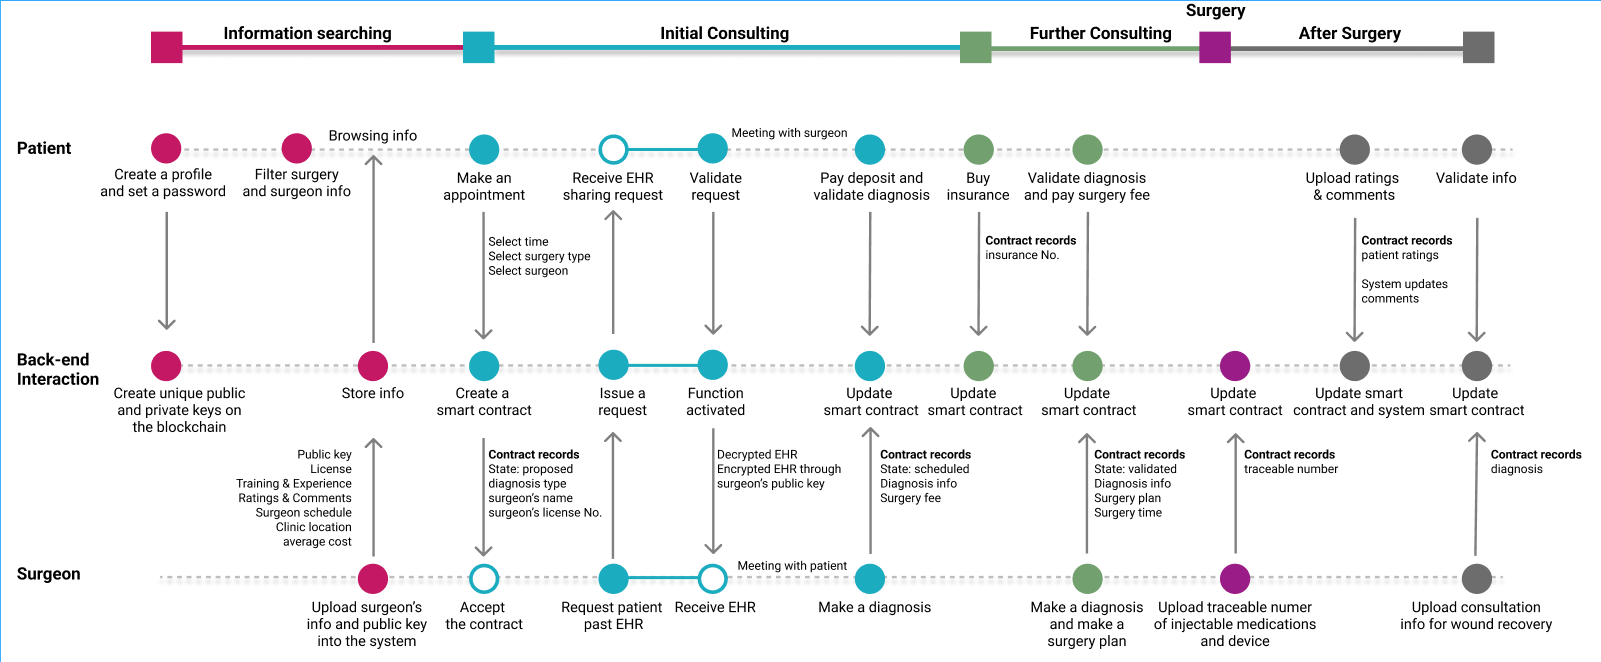
\includegraphics[scale=0.5]{Workflow.jpg}
    \caption{Example of our solution's work flow}
\end{figure}
The workflow between patients and doctors based on our system can be divided into four following stages.
\subsubsection{Information Searching}
In this initial stage, patients and doctors need to create their private-public key pair so that the patient can set up a secure account to store health data and the doctor can become searchable. Then, the patient can search for doctors based on the initial public information stored on the blockchain.
\begin{figure}[H]
    \centering
    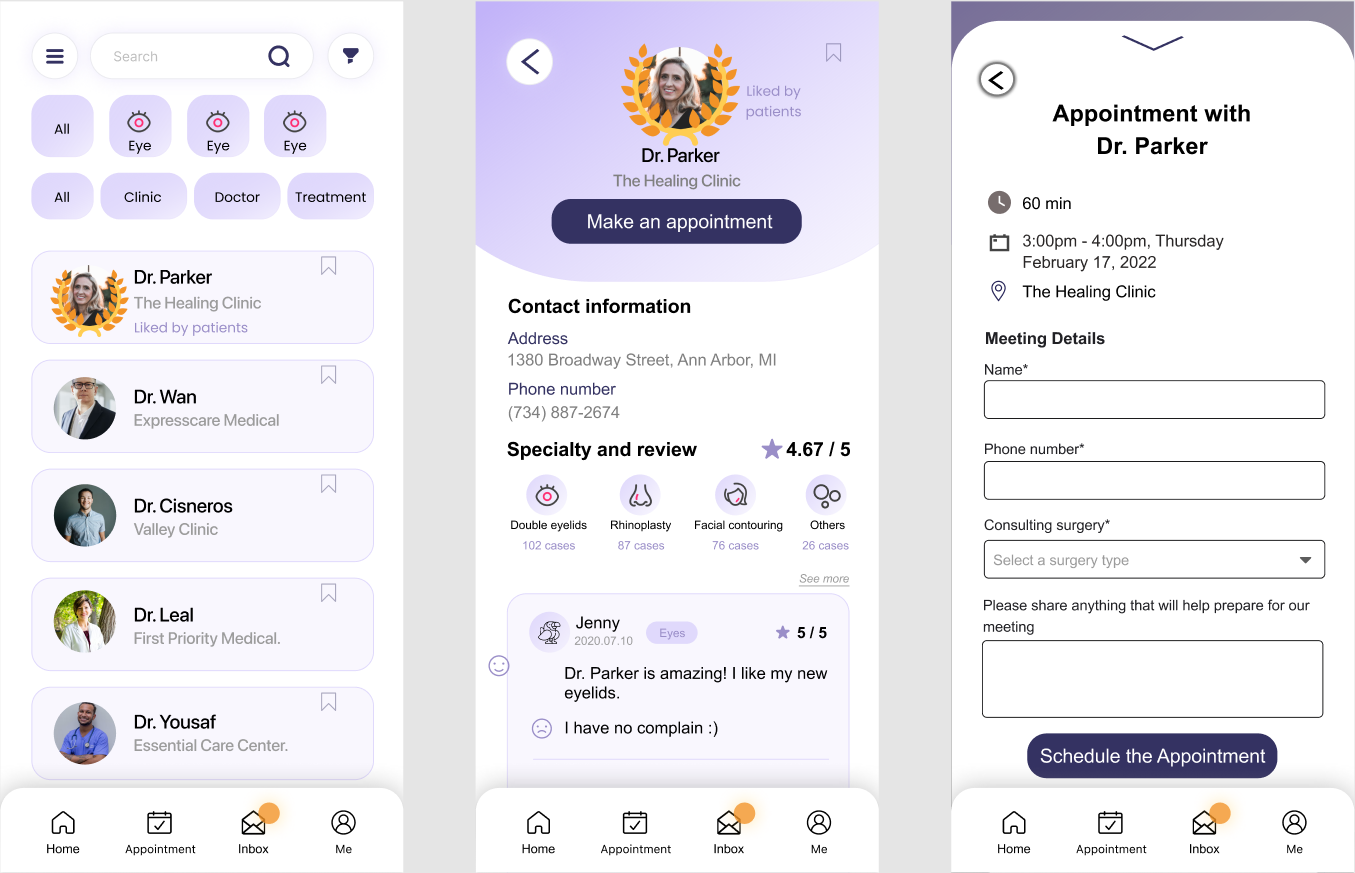
\includegraphics[scale=0.5]{Appointment.jpg}
    \caption{Information Search}
\end{figure}
The searching process is very similar to the existing application, and then the patient can propose a smart contract with an appointment time to the doctor's public address. The creation of a smart contract will cause some transaction fees since it needs to store new data on the blockchain. During the searching process, previous patients' reviews can serve as a reference. Patients can make choices either based on the previous reviews or the smart contract records associated with a specific doctor. Different from the traditional system, it's impossible for the doctor to fake the review because they're linked to a smart contract containing all immutable information regarding the treatment. If the doctor wants to make a fake review, he or she must go through the whole process from proposing a smart contract to the end of visiting, which requires a lot of time and money.
\subsubsection{Initial Consulting}
After receiving the patient's request for the surgery, the doctor can schedule the surgery as well as ask the patient for a deposit. The deposit makes sure that the patient will keep the time and appear at the surgery. In this stage, the doctor can also request to view the patient's previous medical history record. Since the medical history records are stored on the blockchain, only the person with the owner's private key can determine whether to share them. If the patient authorizes the access, the records will be decrypted by the patient's key and encrypted by the doctor's key again so that only the doctor can view them. Since all this process is done through an atomic smart contract, the content of the smart contract can't be revealed to other people.
\par If both doctor and patient agree with the schedule, deposit, and other information stored in the smart contract, they can accept it by putting a digital signature with their own private keys. Since then, the status of the smart contract will be set as \emph{SCHEDULE}, meaning that the doctor and the patient have made a promise that they will have surgery, and the public can know whether they follow the schedule well. At the same time, the deposit will be charged from the patient's account.
\begin{figure}[H]
    \centering
    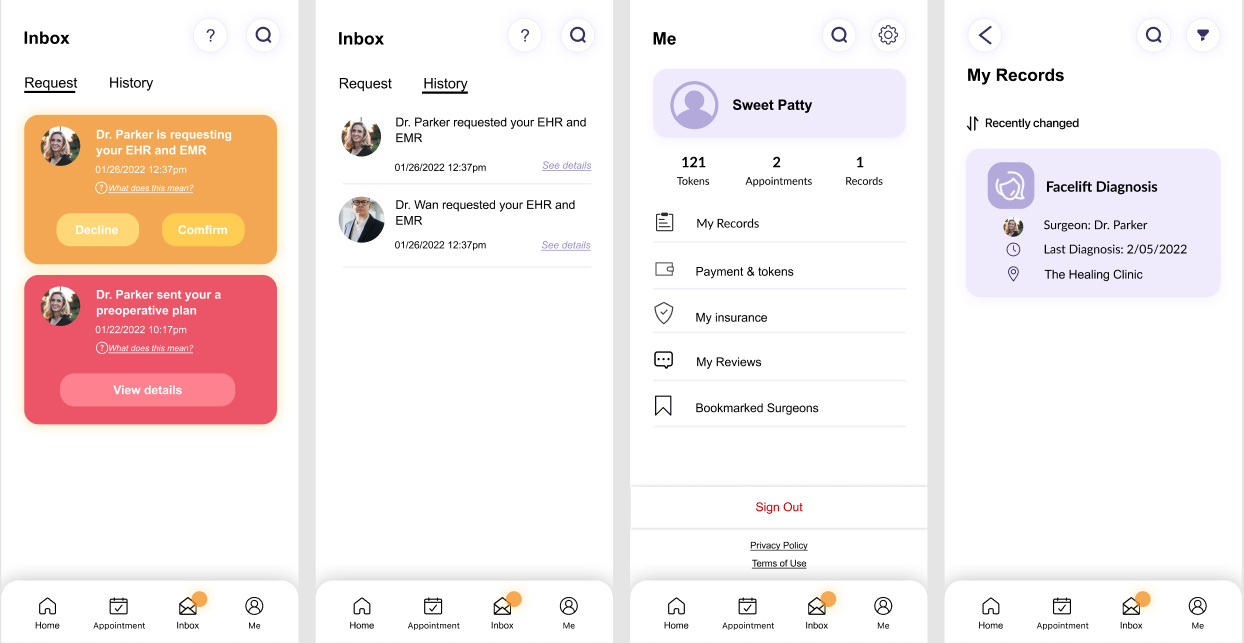
\includegraphics[scale=0.5]{InitialConsulting.jpg}
    \caption{Initial Consulting}
\end{figure}
\subsubsection{Further Consulting}
After the first consultation, doctors and patients should have a plan for the following surgery. In this stage, they need to decide the medicine used for the surgery as well as link the smart contract to the insurance claims with clear terms.
\begin{figure}[H]
    \centering
    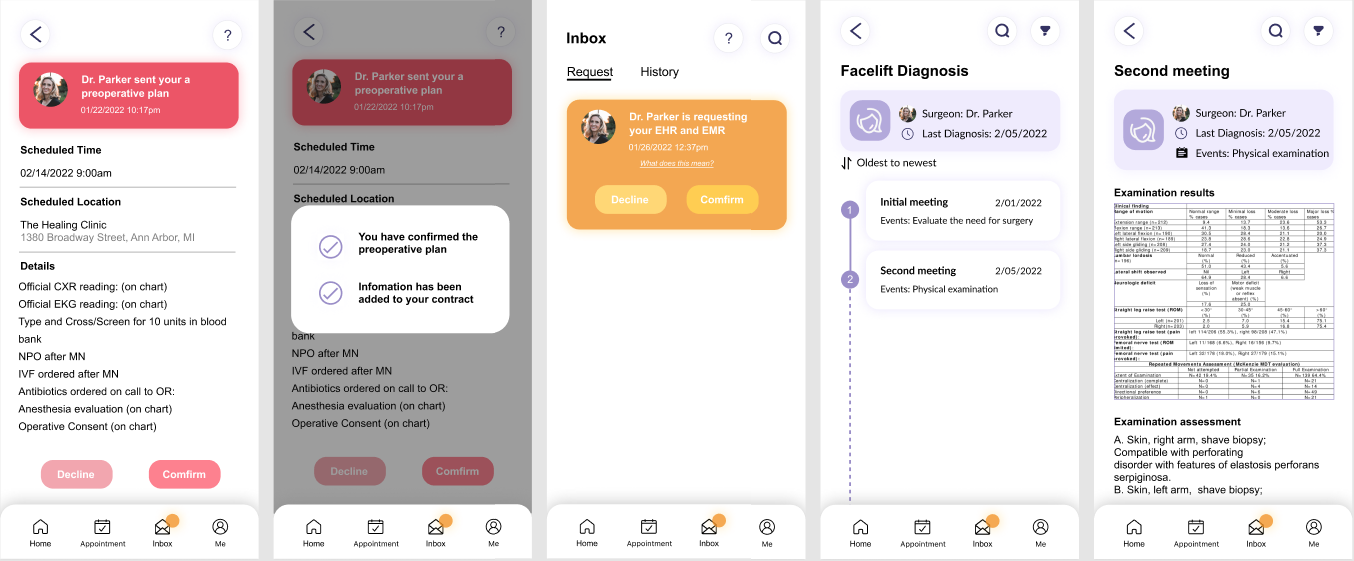
\includegraphics[scale=0.5]{SecondConsulting.jpg}
    \caption{Information Search}
\end{figure}
All valid medicine used in the surgery, such as anesthetics, should be recorded on the blockchain as soon as they're manufactured. Therefore, the doctor and the patient should be able to check the information of the medicine and make sure that it's valid for the surgery. The insurance claims will be written by the insurance company in a smart contract as well. Compared to those written on paper, coded insurance is more clear and there automated, because there is no ambiguity and can be triggered automatically. After this stage, both surgeon and patient need to put a digital signature again and the status of the smart contract will be converted to \emph{CONFIRMED}.
\subsubsection{Surgery}
In this stage, the surgeon is responsible for recording any important information related to the surgery on the smart contract. After the surgery is done, the surgeon can set the smart contract as \emph{EXECUTED}.
\subsubsection{After surgery}
After the surgery, the doctor will encrypt the surgery summary and further prescription with the user's public key and upload the data on the blockchain. Then the patient can check the surgery summary and write a review. If the patient is not satisfied with the summary or the result, then he can write the concern into the review so that it can be referred to other patients. When the review is completed, the patient can set the smart contract as \emph{CLOSED} by putting another digital signature, then the deposit will be transferred to the doctor automatically and the summary will be linked to the user's account. If the surgery's outcome matches any term in the insurance, it'll automatically trigger the claims.
\subsubsection{Accidents}
Neither the surgeon nor the doctor can be sure that everything will go well during the surgery, however, we must have a clear and convincible protocol to deal with it. If an accident happens, the surgeon and doctor should either deal with it with the insurance term or reach an agreement and record the history on the smart contract. Then they need to update the smart contract's state together with their digital signatures. If the accident is far worse, since the doctor's and smart contract's information are public, there should be enough evidence for investigation.
\par Since updating the smart contract requires both patient and surgeon's signature, the surgery can't be closed without everyone being unsatisfied. In this way, previous surgeries can be valid evidence to show how the surgeon is. The better the surgeon is, the more \emph{CLOSED} smart contract with the good review he should have. If there are a large fraction of unclosed smart contracts, then the public can trace the recorded information and see why it's unclosed. With the immutability and authenticity accuracy, the system provides a fair evaluation system for the patients and it encourages the surgeons to behave well. 
\section{Comparsion}
\subsection{Reliable}
Compared to the existing solution, the blockchain-based system is more robust due to its resistance to a single-point failure. To comprise the system, the malicious people need to own much higher resources than is required to attack a traditional database. In addition, cryptography and the hash function used in blockchain systems make sure that nobody can control another's accounts without knowing the private key. Hence, the users don't need to be worried about the security of their data stored on the blockchain. Since medical history records are very sensitive information, this feature is critical for patients. 
\subsection{Functionality}
The blockchain system can work as any existing system. We can easily scan the previous surgery history records and provide a recommendation to the patients. The recommendation algorithm can be open to the public as well so that it can be trusted by anyone. What's more, patients can use the blockchain-based system to do more than traditional systems, such as managing their medical history records or trigger clearly defined insurance claims. As for the review system, since the public can easily trace each review's corresponding surgery status, the reviews are more trustworthy and can help the patients to select the right surgeon for surgery.
\subsection{Compatibility}
Since our solution has much more function, compatibility can be a concern. For example, some patients' medical history records may be stored in the traditional database right now, and it may require a large effort to export them to the blockchain. In addition, traditional insurance terms are too complex to be translated into clear smart contract code. When it comes to disputes, accidents, or claims, people may still prefer human service. However, the system can still work without a fully automated insurance smart contract, we just need to record what happened during the surgery can show it to an insurance company. 
\subsection{Performance}
For now, the prototype is developed on the Ethereum Virtual Machine, which is suffering from high transaction costs as well as latency. The blockchain's performance will be critical for scalability as well as user experience, because patients may not be willing to spend a large amount of extra time or fee for a decentralized system. Luckily, there are a lot of projects aiming at improving the blockchain's performance by using different consensus algorithms such as Algorand\cite{algorand}
\subsection{Acceptance}
Blockchain and cryptocurrency are still a controversial topic all over the world, and the terms like private key and smart contract make blockchain look unapproachable for normal people. To encourage more people to use the blockchain system, more development in the ecosystem is required. On the other hand, a native token is usually issued on the blockchain to smoothen the transactions. For users, the volatility of the token's price can be a concern, and more infrastructures like exchanges may be required.
\section{Conclusion}
In this paper, we have an overview of the current plastic surgery industry as a social business and identify the main issue within it. We look into Zocdoc's existing solution and discuss our concerns. Then we present a system built upon blockchain to record the actions of all stakeholders. The immutability and traceability of the blockchain system make sure that records are authenticated and trustworthy. Hence, these records can be used as reviews and provide references or recommendations for customers to find a reliable surgeon, which is quite helpful to make the industry more transparent. Thanks to cryptography, the system also ensures the security of patients' private data. The smart contract makes the transaction between patients and doctors smoother and enables the automatic execution of insurance claims.
\par We've shown the practicability by developing a prototype and testing on an Ethereum Debug Virtual Machine, but we're looking forward to its potential beyond plastic surgeries. The false-marketing exists on almost every platform with customer reviews. Our blockchain can be an effective method to authenticate these reviews and help the customers make the right choice.
\section{Acknowledgement}
I'm grateful to Joe Ortigara, Noah Chatman, Yue Hu, and Ziwei Chen for their contribution on this idea at University of Michigan. Their efforts for market analysis and prototype development are very helpful.
\bibliographystyle{plain}
\bibliography{Reference}

\end{document}